\documentclass[12pt,a4paper]{scrartcl}
\usepackage[left=4cm,right=2cm, top=3cm, bottom=3cm]{geometry}
\usepackage[T1]{fontenc}
\usepackage[utf8]{inputenc}
\usepackage[ngerman]{babel}
\usepackage{lmodern}
\KOMAoption{listof}{entryprefix}


% =================== - TEXT - =========================
% for header in komascript documents
\usepackage[automark,headsepline]{scrlayer-scrpage}
\clearpairofpagestyles
\pagestyle{scrheadings}
\setkomafont{pageheadfoot}{}
\ihead{\leftmark}
\cfoot*{\pagemark} %Pages for heading and plain pages
\usepackage{enumitem}
\usepackage{hyperref}

% heading spacing
\usepackage[onehalfspacing]{setspace}
\parindent 0pt
\parskip 1.5em
% text symbols
\usepackage{textcomp}
\usepackage{tabto}

% =================== - Tables - =====================
\usepackage{tabularx}
% \usepackage{colortbl, hhline}
\usepackage[table]{xcolor}
% =================== - GRAPHICS - =====================
\usepackage{float}
\usepackage{graphicx}
\usepackage{caption}
\usepackage{subcaption}


% =============== - MUSIC - =========================
\usepackage[chorded]{songs} % Paket fuer Akkorddiagramme
\newcommand{\RomanNumeralCaps}[1]
    {\MakeUppercase{\romannumeral #1}}

% ======================================================
%					- END OF PREAMBLE -
% ======================================================

\begin{document}

% ========= - TITLE AND NONPAGECOUNT SITES - ============
\pagenumbering{Roman}
\begin{titlepage}

    \vspace{20mm}

    \centering
    \huge\textbf{Blues}\par
    \vspace{3mm}

    \begin{figure}[htbp]
        \centering
        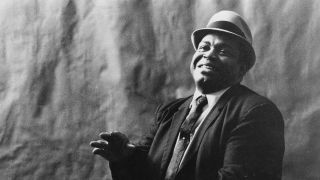
\includegraphics[width=0.8\textwidth]{images/title_img}
    \end{figure}

    \vspace{3mm}
    \textsc{\LARGE{Mathias Gewissen}}\par
    \vspace{3mm}
    \large Untertitel \par

\end{titlepage}
\thispagestyle{plain}
\tableofcontents

% ================= - MAIN TEXT PART - =================

\newpage
\pagenumbering{arabic}
\section{Einleitung}
Die Musiktheorie gliedert sich in Harmonie- und Tonsatzlehre, Analyse, 
Formenlehre, Gehörbildung, Höranalyse, Improvisation und Komposition.
Musiktheorie erklärt, wie Musik funktioniert. Sie ist die Struktur, die einem Song zugrunde liegt und erklärt, wie sie funktionieren. Doch Musiktheorie kann 
auch den Weg nach vorne weisen. Zumindest die Grundlagen der Theorie zu lernen ist ein 
unumgänglicher Teil der musikalischen Entwicklung. Am Anfang kann die Theorie etwas 
einschüchternd wirken. Das Thema ist so groß, dass es schwer ist zu wissen, wo man am 
besten anfängt. Dies ist ein Leitfaden, der dabei hilft, mit der Musiktheorie 
loszulegen, sodass die Grundlagen leicht verstanden werden und sie korrekt auf eigene 
Musik angewendet werden können.
\newpage
\section{Grundlagen}
\subsection{Melodie}
Eine Melodie ist eine \textbf{lineare Sequenz von Tönen}, die von der Person, 
die sie sich anhört, als Einheit wahrgenommen wird. Die Melodie steht im Vordergrund 
eines Songs und besteht aus einer \textbf{Kombination aus Tonhöhe und Rhythmus}. Tonsequenzen, 
die eine Melodie ausmachen, sind musikalisch befriedigend und meistens der einprägsamste 
Teil eines Songs.

Von eingängigen Refrains bis hin zu mitreißenden Gitarrenriffs – Melodien definieren die Musik, 
weil sie Teil der Musik sind, die am ehesten im Gedächtnis bleibt. Dabei ist zu beachten, dass 
es einen Unterschied gibt zwischen Harmonie 
und Melodie: \textbf{Eine Melodie wird zur Harmonie, wenn vollkommen unterschiedliche Töne darüber- oder 
daruntergesetzt werden und alles zur gleichen Zeit gespielt wird}. Auf diese Weise werden Akkorde 
sowie Gesangs- und Instrumental-Harmonien gebildet. Eine gute Melodie zieht die Aufmerksam der 
Zuhörer*innen auf sich und fesselt sie. Songwriter*innen und Komponist*innen nutzen Melodien, 
um Geschichten zu erzählen und dem Publikum etwas zu geben, an das sie anknüpfen und sich erinnern 
können. Die gängigsten Arten, Melodien in der Musik einzusetzen, sind Strophen, Refrains und Bridge-Vocals, 
doch auch Instrumental-Melodien sind wichtig.

Selbst die simpelste Melodie profitiert von unerwarteten Rhythmen. Hier sind ein paar Tipps um Melodien 
eindringlicher und abwechselungsreicher zu gestalten:
\begin{itemize}
    \item \textbf{simpelste Melodien profitieren von unerwarteten Rhythmen}
    \item \textbf{Wenn Melodien immer bei Beat 1 beginnen}: Kann sie kurz davor oder danach beginnen. Selbst die 
    kleinste Veränderung im Rhythmus kann eine Melodie auf subtile, jedoch massive Weise verändern.
    \item \textbf{Melodische Kontur}: Ist die allgemeine Form einer Melodie, d.h. die Art, wie sie sich nach 
    oben und unten bewegt.
    \item \textbf{Bewegung in Melodie}: Bewegung in Sprüngen findet statt, wenn eine Melodie in Intervallen, die 
    größer sind als eine Sekunde, fortschreitet. Allerdings sind zu viele große Sprünge hintereinander schwieriger 
    in eine einzelne melodische Einheit zusammenzufassen.
    \item \textbf{Melodien existieren nicht in einem Vakuum}: Es besteht ein wichtiges Gleichgewicht zwischen der 
    Melodie und ihrer unterschwelligen Harmonie. Die Akkordnoten \textbf{(die Tonleiterschritte 1, 3, 5 und 7)} sind die 
    stärksten und \textbf{stabilsten Plätze, auf denen man landen kann}.
    
\end{itemize}


\subsection{Harmonie}
Harmonien sind wichtige Elemente eines Songs. Sie ist allerdings nicht immer leicht umzusetzen. 
Doch es gibt ein paar Elemente eines Songs, die das Songwriting voranbringen – die Harmonik gehört dazu. 
Egal ob fortgeschrittene*r Musiker*in oder vollkommener Neuling – musiktheoretisches Wissen bietet massive Vorteile.

Harmonien entstehen immer dann, wenn zwei oder mehrere Töne gleichzeitig gespielt werden. \textbf{Harmonik} kann 
sich auf das \textbf{Arrangement individueller Töne bzw. Tonstufen zu einem Akkord sowie auf die allgemeine Akkordstruktur 
eines Musikstücks beziehen}. Doch in der Musiktheorie bezieht sich Harmonik normalerweise auf das Bilden 
von Akkorden, die Eigenschaften von Akkorden und Akkordfolgen.

\begin{itemize}
    \item \textbf{Tonstufe}: ist ein einzelner Ton einer diatonischen Tonleiter. Als Kernbestand des abendländischen 
    Tonsystems kann man die sieben Tonstufen \textbf{C, D, E, F, G, A und H ansehen, die Stammtöne.} Die Tonstufen 
    einer gegebenen Tonleiter werden mit lateinischen Ordinalzahlen benannt.
\end{itemize}

\begin{table}[H]
    \caption{Tonstufen C-Dur Tonleiter}
    \begin{tabularx}{\textwidth}{|>{\hsize=.2\hsize}X|>{\hsize=.4\hsize}X|>{\hsize=.4\hsize}X|}
    \hline
    Tonstufe & Ton & lateinische Ordinalzahlen\\ \hline
    \textbf{1} & \textbf{C} & \textbf{Prime} \\ \hline
    2 & D & Sekunde \\ \hline
    3 & E & Terz \\ \hline
    4 & F & Quarte \\ \hline
    5 & G & Quinte\\ \hline
    6 & A & Sexte \\ \hline
    7 & H & Septime \\ \hline
    \textbf{8} & \textbf{C} & \textbf{Oktave}\\ \hline   
    9 & D & None\\ \hline   
    10 & E & Dezime\\ \hline   
    11 & F & Undezime\\ \hline   
    12 & G & Doudezime\\ \hline   
    12 & A & Terzdezime\\ \hline   
    \end{tabularx}
\end{table}

Harmonik wird durch römische Ziffern repräsentiert. Der Name eines Akkords wird durch eine römische Ziffer
ersetzt. Und zwar \textbf{die Ziffer die der Tonstufe seines Grundtons entspricht}. Römische Ziffern geben an, 
zu welcher harmonischen Kategorie ein Akkord gehört. Und Akkord-Kategorien bestimmen die Funktion eines 
Akkords innerhalb eines Musikstücks. In der tonalen Musik gibt es drei funktionale Kategorien:

\begin{itemize}
    \item \textbf{Tonika}: Tonika-Akkorde sind Ruhezonen, bei denen einem die harmonische Aktion eines 
    Songs am stabilsten vorkommt.
    \item \textbf{Dominante}: Dominant-Akkorde stellen eine Art Gegenteil zu den Tonika-Akkorden dar. 
    Bei diesem Akkord will die vierte und siebte Tonleiterstufe auf natürliche Weise nach unten 
    (vierte-dritte) und nach oben (siebte-Tonika) rücken, um den Tonika-Akkord aufzulösen.
    \item \textbf{Prädominante}: Die anderen Akkorde in dem harmonischen Vokabular sind die Prädominanten, 
    mit denen die Lücke zwischen Stufe I und Stufe V überbrückt wird.

\end{itemize}


\subsection{Rhytmus}

\subsection{Tonleitern}
Eine Tonleiter oder Ton-Skala ist in der Musik eine Reihe von der Tonhöhe nach geordneten Tönen, 
jenseits derer die Tonreihe in der Regel wiederholbar ist. In den meisten Fällen hat eine Tonleiter 
den Umfang einer Oktave. Weit verbreitet sind diatonische Tonleitern in Dur und Moll oder die 
Kirchentonleitern. Tonleitern sind durch Tonabstände definiert.

\begin{figure}[htbp]
    \centering
    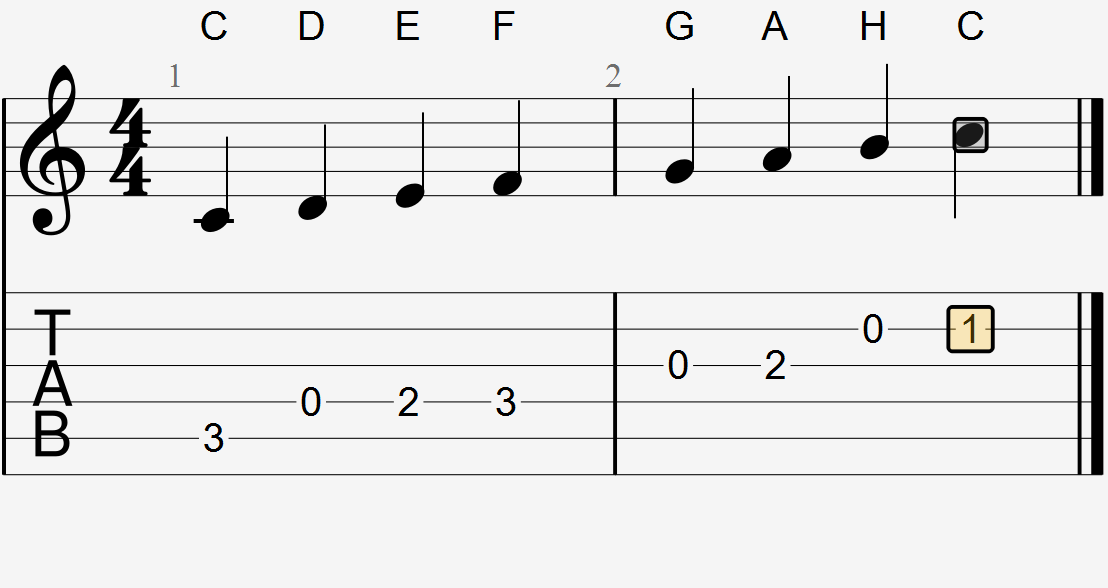
\includegraphics[width=0.8\textwidth]{images/C_Dur_Tonika}
\end{figure}

\subsection{Akkorde}
\RomanNumeralCaps{1}
\RomanNumeralCaps{2}
\RomanNumeralCaps{3}
\RomanNumeralCaps{4}
\RomanNumeralCaps{5}
\RomanNumeralCaps{6}
\RomanNumeralCaps{7}

\subsection{Tonarten}
\subsubsection{subsubsection}



\end{document}